
\section{Evaluation}
\label{sect:exper}

We have implemented a prototype of the parititon-based deduplication scheme based on the 
Alibaba's cloud platform.  Objectives of our experimental evaluation are:
1) Analyze the commonality of content data blocks and the popularity  of hot items. 
2) Assess the effectiveness  of 3-level deduplication for reducing the storage cost of snapshot 
backup. 
3) Examine the impacts of CDS size on deduplication ratio.

\subsection{Experimental setup}

At Aliyun our target is to backup cluster up to 1000 nodes
with 25 VMs on each.
%We are running our deduplication/backup  service on 100 nodes.
%Memory usage is about 150MB space per node during backup and
%the CPU usage is very small during the experiments. 
Based on the data studied,  each VM has about  40GB of storage  data usage on average,
OS disk and data disk each takes about 50\% of storage space.
The backup of VM snapshots is completed within two hours every day,
and that translates to a backup throughput of 139GB per second, or 500TB per hour.
For each VM, the system keeps 10 automatically-backed snapshots in the storage while
a user may instruct extra snapshots to be saved.

% the system must finish saving daily snapshots of all VMs in 2 hours. In our typical 1000 nodes cluster, each node hosts 25 VMs, each VM has 40GB of data on average, that translates to backup throughput of 139GB/second, or 500TB/hour.

%In our snapshot deduplication architecture, CDS is the key to achieve greater deduplication than
%incremental backup solutions. Our basic assumption of CDS us that VM disks, especially OS disks,
%have huge amount of data in common, and such common data can be represented by a relatively smaller data set
%because of their high appearence frequency. As a result, the major portion of snapshot deduplication effect shall 
%emerge from eliminating the duplication of such a small data set. In this section, we evaluate
%the effectiveness of CDS using real user VM disks from our production VM cluster.

Since it's impossible to perform large scale analysis without affecting the VM performance,
we sampled two data sets from real user VMs to measure the effectiveness of our deduplication scheme.
Dataset1 is used study the detail impact of 3-level deduplication process,
it compose of 35 VMs from 7 popular OSes: 
Debian, Ubuntu, Redhat, CentOS, Win2003 32bit, win2003 64 bit and win2008 64 bit. For each OS, 
5 VMs are chosen, and every VM come with 10 full snapshots of it OS and data disk. 
The overall data size for this 700 full snapshots is 17.6 TB.

Dataset2 contains the first snapshots of 1323 VMs' data disks from a small cluster with 100 nodes. 
Since inner-VM deduplication is not involved in the first snapshot, this data set helps us to 
study the CDS deduplication against user-related data. The overall size of dataset2 is 23.5 TB.

All data are divided into 2 MB fix-sized segments and each segment is divided into 
variable-sized content blocks ~\cite{similar94,rabin81} with an average size of 4KB.
The signature for variable-sized blocks is computed using their SHA-1 hash. 
Popularity of data blocks are collected through global counting 
and the top 1\% will fall into CDS, as discussed in Section~\ref{sect:crossVM}.

\comments{
a storage dataset of 1323 VM users collected from 100 Aliyun's cloud nodes to evaluate the effectiveness.
In this dataset, there are 10 snapshots per each VM user and the total amount of space investigated 
is 23.5 terabytes.
Each VM file is  divided into content blocks of
variable sizes~\cite{similar94,rabin81} with an average size of 4KB. 
The signature for variable-sized blocks is computed using  their SHA-1 hash. 
Each segment is of size 2MB.  
Popularity is computed by using 90\% of dataset, which reflects our setting that the system recomputes
CDS every 1-2 days to catch up the popularity trend.
}
%seg, and we performed global perfect deduplication 
%to caculate the number of duplicate copies of each individual unique block. We choose 2KB, 4KB, 16KB as the minimum, average
%and maximum block size
%OS data
%user data: zipf
%prediction
%say something about aliyun


%To compare the effectiveness with a full deduplication approach with an approximation,
%we use  extreme binning and perfect deduplication~\cite{extreme_binning09}. 
%For perfect deduplication and extreme binning, each snapshot is also divided into chunk blocks
%using TTTD with an average size of 4KB. The original extreme binning work uses the whole file
%as the input unit and  this size is too big in our system. 
%Thus we split each image snapshot file into variable-sized segments base on the block hash list, 
%using TTTD with average size of 2MB.

\subsection{Effectiveness of 3-level Deduplication}

%\begin{figure}
%  \centering
%  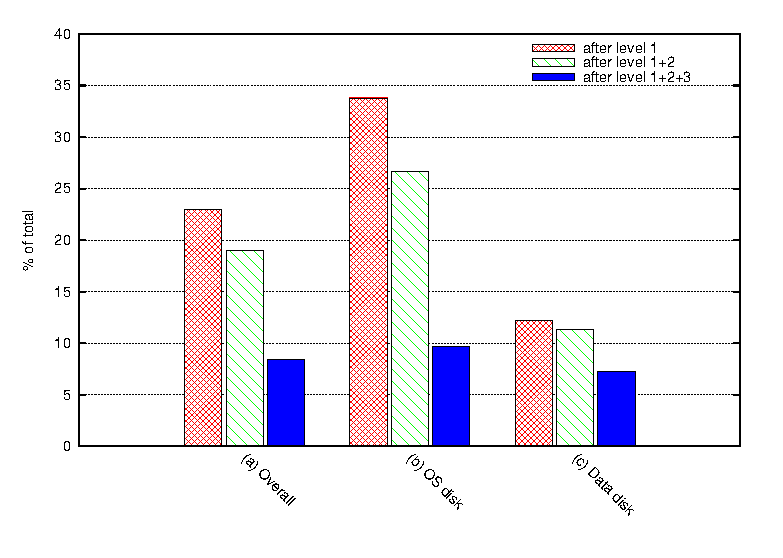
\epsfig{file=images/overall_effect.eps, width=3.5in}
%  \caption{Impacts of 3-level deduplication. The height of each bar is the data size after 
%deduplication divided by the original data size and the unit is percentage. }
%
%  \label{fig:overall}
%\end{figure}

Figure~\ref{fig:overall} shows the overall impact of 3-level deduplication on dataset1.
The X axis shows the overall impact in (a),  impact on OS disks in (b), and impact on data disks in (c).
Each bar in the Y axis shows the data size after deduplication divided by the original data size.
Level-1 elimination can reduce the data size to about 23\% of original data, namely it delivers close 77\% reduction.
Level-2 elimination is applied to data that could pass level-1, it
reduces the size further to about 18.5\% of original size, namely it delivers additional 4.5\% reduction.
Level-3 elimination together with level 1 and 2
reduces the size further to 8\% of original size, namely it delivers additional 10.5\% reduction.
Level 2 elimination is more visible in OS disk than data disk, because data change frequency is really small
when we sample last 10 snapshots of each user in 10 days. Nevertheless, the overall impact of level 2 is still significant.
A 4.5\% of reduction from the original data represents about 450TB space saving for a 1000-node cluster.


%\begin{figure}
%  \centering

%  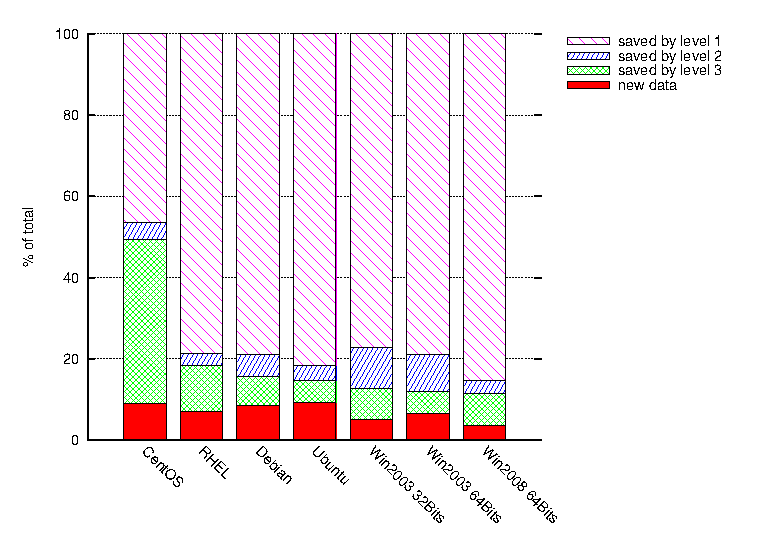
\epsfig{file=images/3level_os.eps, width=3.5in}
%  \caption{Impact of 3-level deduplication for OS releases.}
%  \label{fig:oscds}
%\end{figure}

%To see the impact of multi-level deduplication on different OS releases,
%Some of  OS disks are modified frequently and in some cases,  users even store a large amount of user data on
Figure~\ref{fig:oscds} shows the impact of different levels of deduplication for different OS releases.
In this experiment, we tag each block in 350 OS disk snapshots from dataset1 as  ``new''
if this block cannot be deduplicated by our scheme and thus has to be written to the snapshot store;
``CDS''  if this block can be found  in CDS;
``Parent segment'' if  this block is marked unchanged in parent's segment recipe.
``Parent block'' if  this block is marked unchanged in parent's block recipe.
With this tagging, we compute the percentage of deduplication accomplished by each level.
As we can see from Figure~\ref{fig:oscds}, level-1 deduplication accomplishes a large percentage of elimination,
this is because the time interval between two snapshots in our dataset
is quite short and the Aliyun cloud service makes a snapshot  everyday  for each VM.
On the other hand,  CDS still finds lots of duplicates that inner VM deduplication can't find,
contributing about 10\% of reduction on average.

It is noticeable that level-1 deduplication doesn't work well for CentOS, a significant percentage of data is not
eliminated until they reach level-3. It shows that even user upgrade his VM system heavily and frequently
such that data locality is totally lost, those OS-related data can still be identified at level-3. 

In general we see a stable data reduction ratio for all OS varieties, ranging from 92\% to 97\%, that means
the storage cost of 10 full snapshots combined is still smaller than the original disk size. And compare to 
today's widely used copy-on-write snapshot technique, which is similar to our level-1 deduplication, our
solution cut the snapshot storage cost by 64\%.



%\begin{figure}
%\centering
%\includegraphics[width=0.45\textwidth]{websearch.pdf}
%\caption{ PDF-based figure.}
%\label{fig:websearch}
%\end{figure}

%\begin{table}[hbt]
%\caption{ Projected enrollment for the first five years.}
%\begin{center}
%\begin{tabular} {|c|c|c|c|c|c|}
%\hline  & Year 1 & Year 2 &Year 3 & Year 4 & Year 5 \\
%\hline Enrollment & 10&  15 & 20 & 25 & 30 ( $\le$ 40)\\
%\hline
%\end{tabular}
%\end{center}
%\label{tab:enrollment}
%\end{table}

\begin{verbatim}
partition q/machine=		50	100	250	500	1000	2000
Step 1
Seek cost  for accumulating (option1)	0.015972222	0.031944444	0.079861111	0.159722222	0.319444444	0.638888889
Seek for accumlation (option 2)     1.064814815	2.12962963	5.324074074	10.64814815	21.2962963	42.59259259

Step 2
Memory for index+bucket 	0.276	0.138	0.0552	0.0276	0.0138	0.0069
Global index portion		0.23	0.115	0.046	0.023	0.0115	0.00575

buffering factor 			-9.723320158	-8.537549407	-4.980237154	0.948616601	12.80632411	36.52173913
Seek for writing dup sum per VM	-0.000357103	-0.0008134	-0.003486001	0.036603009	0.005422668	0.00380291
\end{verbatim}


%Combining OS disks in all the VMs, we see the overall 7.4TB of data is reduced to 512GB. 
%The extreme binning approach can reduce this data set to 542GB, which is slightly worse. As a reference, 
%perfect deduplication achieves 364GB in this experiment.

%Overall speaking, inner   VM deduplication or  CDS-based deduplication
%can work well alone, but by combining them together we get a fairly good and stable deduplication ratio to 
%all kind of OSes. 
%Compared to a traditional dirty bit approach based on pages of
%each file (e.g. segment in our scheme),
%our CDS-based level 3 approach  can save additional 50\% storage space because many of level 2 block
%content can be eliminated using the CDS also.

